\section{Conclusion}

\begin{figure}[t!]
	\centering
	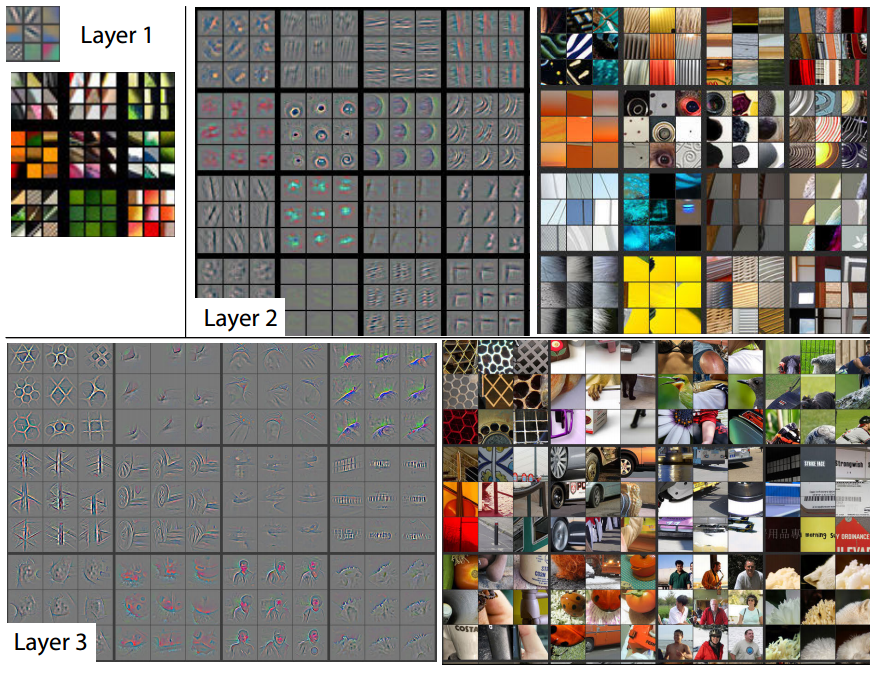
\includegraphics[scale=0.625]{images/filters}
	\caption{Taken from \cite{ZeilerFergus:2013}, this figure shows a selection of features across several layers of a fully trained convolutional network using the visualization technique discussed in section \ref{sec:understanding-convolutional-networks}.}
	\label{fig:feature-activations}
\end{figure}
In the course of this paper we discussed the basic notions of both neural networks in general and the multilayer perceptron in particular. With deep learning in mind, we introduced supervised training using gradient descent and error backropagation as well as unsupervised training using auto encoders. We concluded the section with a brief discussion of regularization methods including dropout \cite{HintonSrivastavaKrizhevskySutskeverSalakhutdinov:2012} and unsupervised pre-training.

We introduced convolutional neural networks by discussing the different types of layers used in recent implementations: the convolutional layer; the non-linearity layer; the rectification layer; the local contrast normalization layer; and the pooling and subsampling layer. Based on these basic building blocks, we discussed the traditional convolutional neural networks \cite{LeCunBoserDenkerHenderson:1989} as well as a modern variant as used in~\cite{KrizhevskySutskeverHinton:2012}.

Despite of their excellent performance \cite{KrizhevskySutskeverHinton:2012, CiresanMeierSchmidhuber:2012}, the internal operation of convolutional neural networks is not well understood \cite{ZeilerFergus:2013}. To get deeper insight into their internal working, we followed \cite{ZeilerFergus:2013} and discussed a visualization technique allowing to backproject the feature activations of higher layers. This allows to further evaluate and improve recent architectures as for example the architecture used in \cite{KrizhevskySutskeverHinton:2012}.

Nevertheless, convolutional neural networks and deep learning in general is an active area of research. Although the difficulty of deep learning seems to be understood \cite{Bengio:2009,GlorotBengio:2010,ErhanManzagolBengioVincent:2009}, learning feature hierarchies is considered very hard \cite{Bengio:2009}. Here, the possibility of unsupervised pre-training had a huge impact and allows to train deep architectures in reasonable time \cite{Bengio:2009,ErhanBengioCourvilleManzagolVincentBengio:2010}. Nonetheless, the reason for the good performance of deep neural networks is still not answered fully.

% The different layers present in recent convolutional networks were introduced in section three. Based on these basic building blocks, we discussed the traditional convolutional neural networks as proposed in \cite{LeCunBoserDenkerHenderson:1989} as well as a more recent implementation as described in \cite{KrizhevskySutskeverHinton:2012}.

% Based on the deconvolutional neural networks, as introduced in \cite{ZeilerKrishnanTaylorFergus:2010}, the authors of \cite{ZeilerFergus:2013} propose a visualization technique allowing to backproject feature activations of higher layers onto the image plain. This allows to get deeper insights into the operation of deep convolutional neural networks.

% Still, training deep architectures is considered a challenge in machine learning \cite{Bengio:2009}. Although, convolutional neural networks can be seen as exception -- as deep convolutional networks are more easily trained due to their constrained architecture --, understanding deep learning is currently a promising research area. In addition, deep architectures allow to learn complex, task specific features (SOURCE) where they would have been handcrafted before. 

% In 2006, the work in \cite{HintonOsindero:2006} is considered as breakthrough in deep learning, as it allows to pre-train deep networks in an unsupervised fashion. Using unsupervised pre-training, deep networks can be trained with traditional methods as gradient descent and the error backpropagation algorithm.

% Nevertheless, the internal operation of higher layers in both convolutional networks as well as general neural networks are not well understood. Here, the work in \cite{ZeilerFergus:2013} allows to visualize feature activations of higher layers and, thus, allows to get more insight into the internal operations. Based on the visualization, architectures can be adapted to give better performance or generalization as well as better training speed.